\section{Price response functions}\label{sec:response_functions}

In Sect. \ref{subsec:response_function_trade} we analyze the responses
functions in trade time scale and in Sect.
\ref{subsec:response_function_physical} we analyze the responses functions in
physical time scale.


%%%%%%%%%%%%%%%%%%%%%%%%%%%%%%%%%%%%%%%%%%%%%%%%%%%%%%%%%%%%%%%%%%%%%%%%%%%%%%%
\subsection{Response functions on trade time scale}
\label{subsec:response_function_trade}

The price response function in trade time scale is defined as
\cite{my_paper_response_financial}
\begin{equation}\label{eq:response_functions_trade_scale_general}
    R^{\left(\textrm{t}\right)}_{i}\left(\tau\right)=\left\langle
    r^{\left(\textrm{t}\right)}_{i}\left(t-1,\tau \right)
    \varepsilon_{i}^{\left(\textrm{t}\right)}
    \left(t, n\right)\right\rangle _{T}.
\end{equation}
To compute the response functions on trade time scale, we use both, the trade
signs and the returns from the tick-by-tick original data during a week in
market time. Then, the response is averaged by the number of trades.

\begin{figure}[htbp]
    \centering
    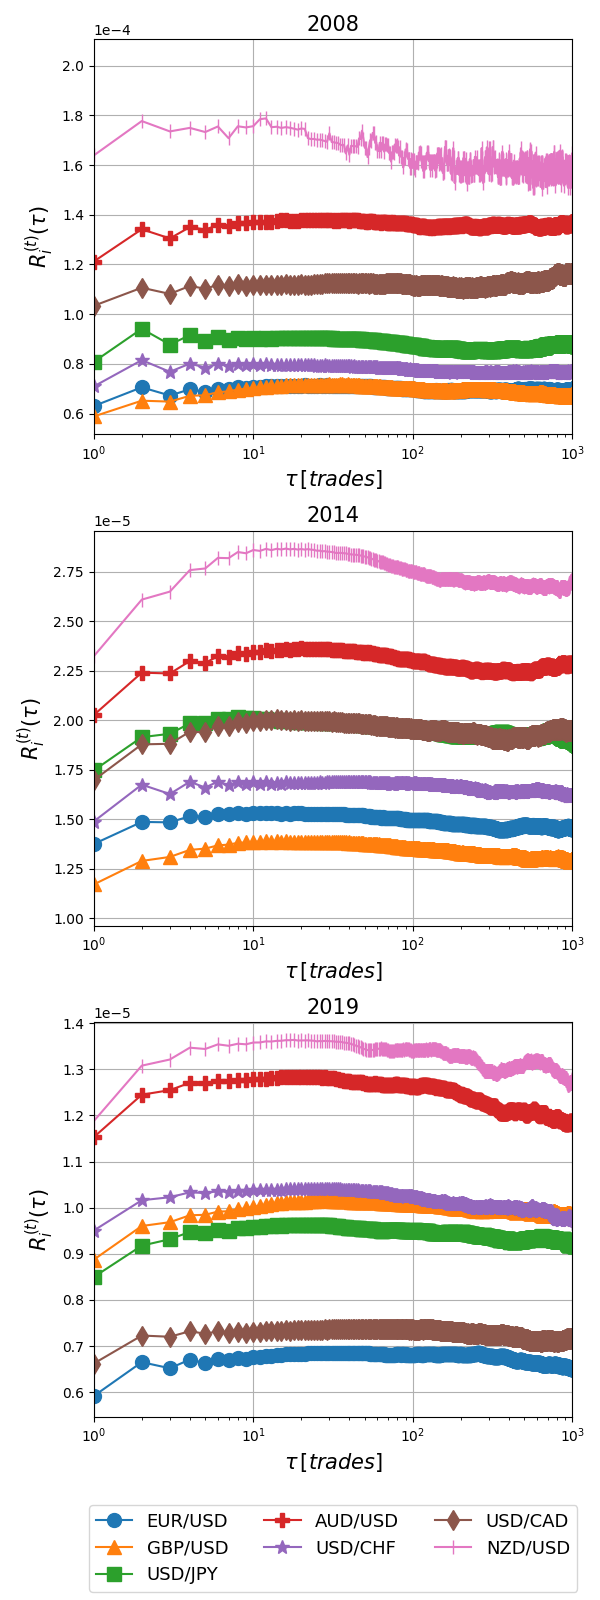
\includegraphics[width=\columnwidth]
    {figures/04_responses_trade_scale.png}
    \caption{Price response functions
             $R^{\left(\textrm{t}\right)}_{ii}\left(\tau\right)$ versus time
             lag $\tau$ on a logarithmic scale in trade time scale for the
             years 2008 (top), 2014 (middle) and 2019 (bottom).}
    \label{fig:response_function_trade_scale}
\end{figure}

The results of Fig. \ref{fig:response_function_trade_scale} show the
price response functions of the seven foreign exchange major pairs used in the
analysis (see Table \ref{tab:majors}) for three different years. The results
found for all the years are entirely in line with price responses seen in other
financial markets, particularly with correlated financial markets. The response
functions have an initial increasing trend to a maximum, that flattens out and
saturates at some level, to then slowly decrease. The shape of the price
response function can be qualitatively explain considering that there is an
initial increase of the response function caused by the autocorrelated
transaction flow, while the flattening out is due to market liquidity adapting
to this flow and thus assuring diffusive prices. For our selected pairs, a time
lag of $\tau = 10^{3} $ trades is enough to see an increase to a maximum
followed by a decrease. Thus, the trend in the price response functions is
eventually reversed. The response signal is much more noisier in the year 2008
for the first seconds in the time lag. This behavior is because of the smaller
amount of data of the corresponding year. In general, more data was recorded in
recent years than in past years. In the three years analyzed, the more liquid
currency pairs have a smaller response in comparison with the non-liquid pairs.
The strength of the response function vary from one year to the other. In 2008
the strength of the signal is one order of magnitude stronger than the response
in 2014, but the signals in 2014 have approximately twice the strength the
signals of 2019. This behavior can be explained by the fact that in recent
times algorithm trading has been used intensively. Thus, many more trades were
carried out in the last years, which means, the impact of each trade is
reduced, and then the response functions tend to decrease compared with
previous years.

%%%%%%%%%%%%%%%%%%%%%%%%%%%%%%%%%%%%%%%%%%%%%%%%%%%%%%%%%%%%%%%%%%%%%%%%%%%%%%%
\subsection{Response functions on physical time scale}
\label{subsec:response_function_physical}

One important detail to compute the price response function on physical time
scale is to define how the averaging of the function will be made, because the
response functions highly differ when we include or exclude
$\varepsilon^{\left(\textrm{p}\right)}_j \left( t\right) = 0$
\cite{Wang_2016_cross}. The price responses including
$\varepsilon^{\left(\textrm{p}\right)}_j \left( t\right) = 0$ are weaker than
the excluding ones due to the omission of direct influence of the lack of
trades. However, either including or excluding
$\varepsilon^{\left(\textrm{p}\right)}_j \left( t\right) = 0$ does not change
the trend of price reversion versus the time lag, but it does affect the
response function strength \cite{Wang_2016_avg}. For a deeper analysis of the
influence of the term
$\varepsilon^{\left(\textrm{p}\right)}_j \left( t\right) = 0$ in price response
functions, we suggest to review Refs. \cite{Wang_2016_avg,Wang_2016_cross}. We
will only take into account the price response functions excluding
$\varepsilon^{\textrm{p}}_j \left( t\right) = 0$.

We define the price response functions on physical time scale, using
the trade signs and the returns sampled in seconds from the original data in
physical time scale. The price response function on physical time scale is
defined as \cite{my_paper_response_financial}
\begin{equation}\label{eq:response_functions_time_scale_general}
    R^{\left(\textrm{p}\right)}_{i}\left(\tau\right)=\left\langle
    r^{\left(\textrm{p}\right)}_{i}\left(t-1, \tau\right)
    \varepsilon_{i}^{\left(\textrm{p}\right)} \left(t\right)\right\rangle _{P}
\end{equation}
\begin{figure}[htbp]
    \centering
    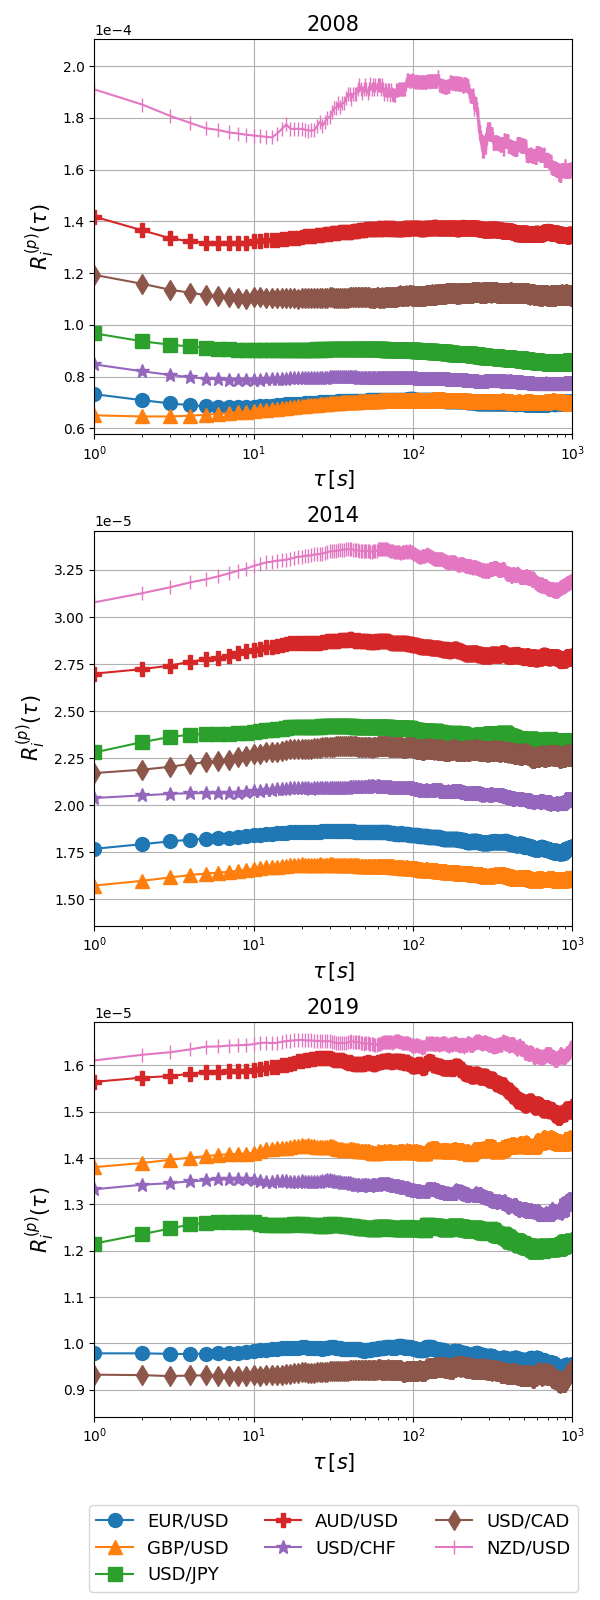
\includegraphics[width=\columnwidth]
    {figures/04_responses_physical_scale.png}
    \caption{Price response functions
             $R^{\left(\textrm{p}\right)}_{ii}\left(\tau\right)$ excluding
             $\varepsilon^{\left(\textrm{p}\right)}_{i}\left(t\right) = 0$ versus time
             lag $\tau$ on a logarithmic scale in physical time scale for the
             years 2008 (top), 2014 (middle) and 2019 (bottom).}
    \label{fig:response_function_physical_scale}
\end{figure}
The results shown in Fig. \ref{fig:response_function_physical_scale} are the
price response functions on physical time scale for three different years. The
results show approximately the same behavior observed in currency exchange
pairs in trade time scale, and in correlated financial markets, where we can
see that an increase to a maximum is followed by a decrease. Thus again, the
trend in the price responses is eventually reversed. An exception occurs in the
year 2008, where the response at short time lags seems to decrease, to then
start to slightly increase, and finally it decrease again.

The price response functions on physical time scale are smoother than the
responses on trade time scale. As we reduce from trade data all the returns and
trade signs in one second to one data point on physical time scale, and as this
sampling gives the same weight to every data point, the curves look smoother.

Compared with the response functions on trade time scale, the strength of the
signal of the response functions on physical time scale are similar in
magnitude in the corresponding years. Thus, the strength of the signal in 2008
for trade time scale is similar to the strength of the signal in 2008 for
physical time scale, and so on. This behavior is different to the one presented
in correlated financial markets, where the results differ about a factor of
two depending on the time scale.

On physical time scale, we can see that the liquid pairs have a smaller price
response compared with non-liquid pairs. Therefore, the price response of a
foreign exchange pair with large activity is smaller to the small impact of
each trade. Also, the older the response, the stronger the signal. We consider
the same argument of algorithm trading to explain why the signals in recent
years are weaker than in older years.
